\section{Histogram data}
In an increasing number of experiments, the data is not anymore collected in a hit-to-hit fashion, but rather as shot-to-shot histograms. For instance, in the case of short and intense laser or (X-)FEL pulses. Rather than individual pulses with e.g. a position and time of impact, the incoming data consists of histograms of \emph{all} hits masses, X-positions, and Y-positions in an event. 

The data treatment could then for instance involve only the visualization of those histograms, or a covariance treatment. The data will be stored in a different way.

TODO

\subsection{Normalization}

In case of histogram data, the amount of counts one often depends on external factors,  for example the measurement time, the FEL power of each shot, the amount of ions present in the trap, their spatial distribution, and possibly
fluctuations in the ESI source. Therefore, this signal needs to be normalized before one can deduct conclusions on the system under study. 

\paragraph {Total ion count} 
When normalizing on the total measured counts, namely all fragments and the ion
parent, the relative intensity might be interpreted as a relative yield. This type of normalization
makes the signal still dependent on:
\begin{itemize}
\item The overlap of FEL with the ions in the trapped volume
\item The FEL light intensity
\end{itemize}
Note that both these aspects can fluctuate over time and thereby influence the normalized ion yield.

\paragraph{Single-histogram mass spectra}
In other experiments, the output data is contained in a single histogram as a (mass) spectrum, but as a function of a changing parameter such as photon energy. The normalization method can be chosen to integrate across different `variables', such as mass and photon energy. 

TODO.

\begin{figure}[h!]
	\centering
	\begin{subfigure}{.25\textwidth}
		\centering
		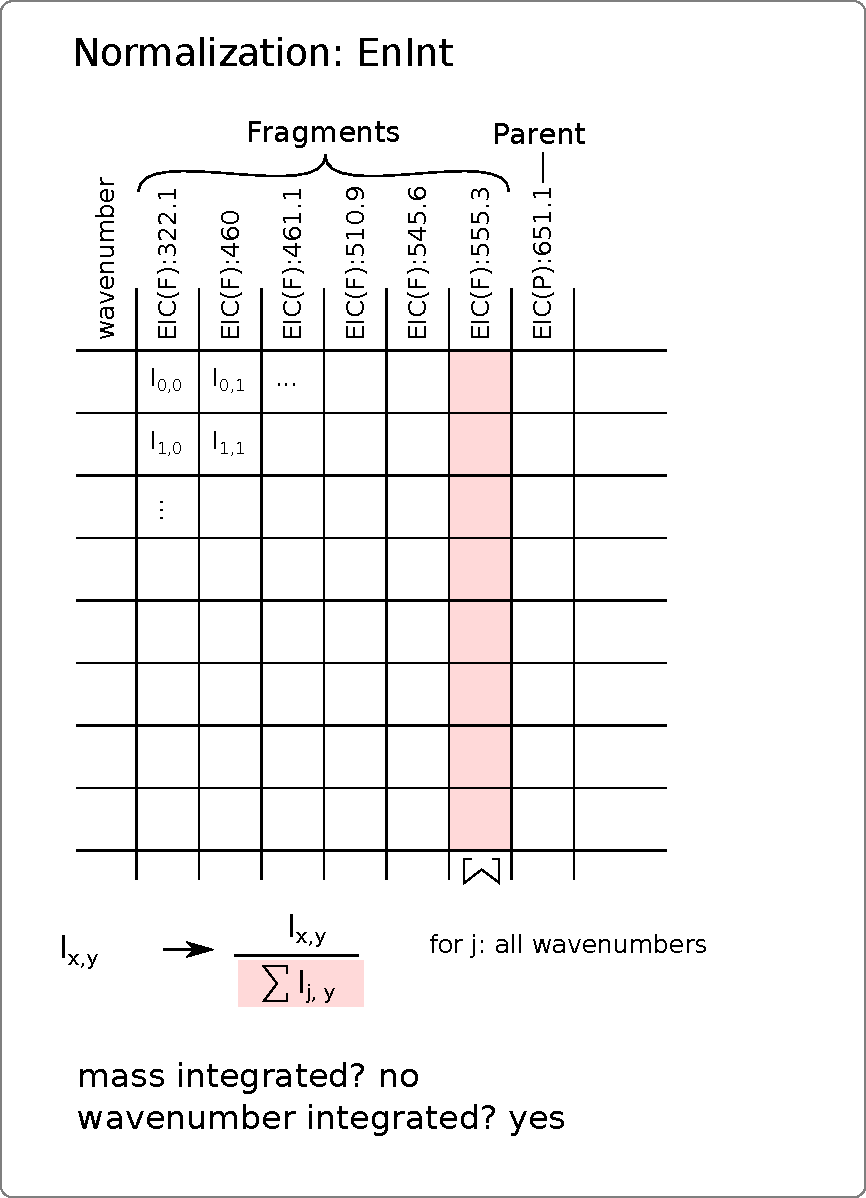
\includegraphics[width=1\linewidth]{../Graphics/Normalization/Normalization_visual_EnInt.pdf}
		\label{fig:MetEnk_sequence_notation}
	\end{subfigure}
	\begin{subfigure}{.25\textwidth}
		\centering
		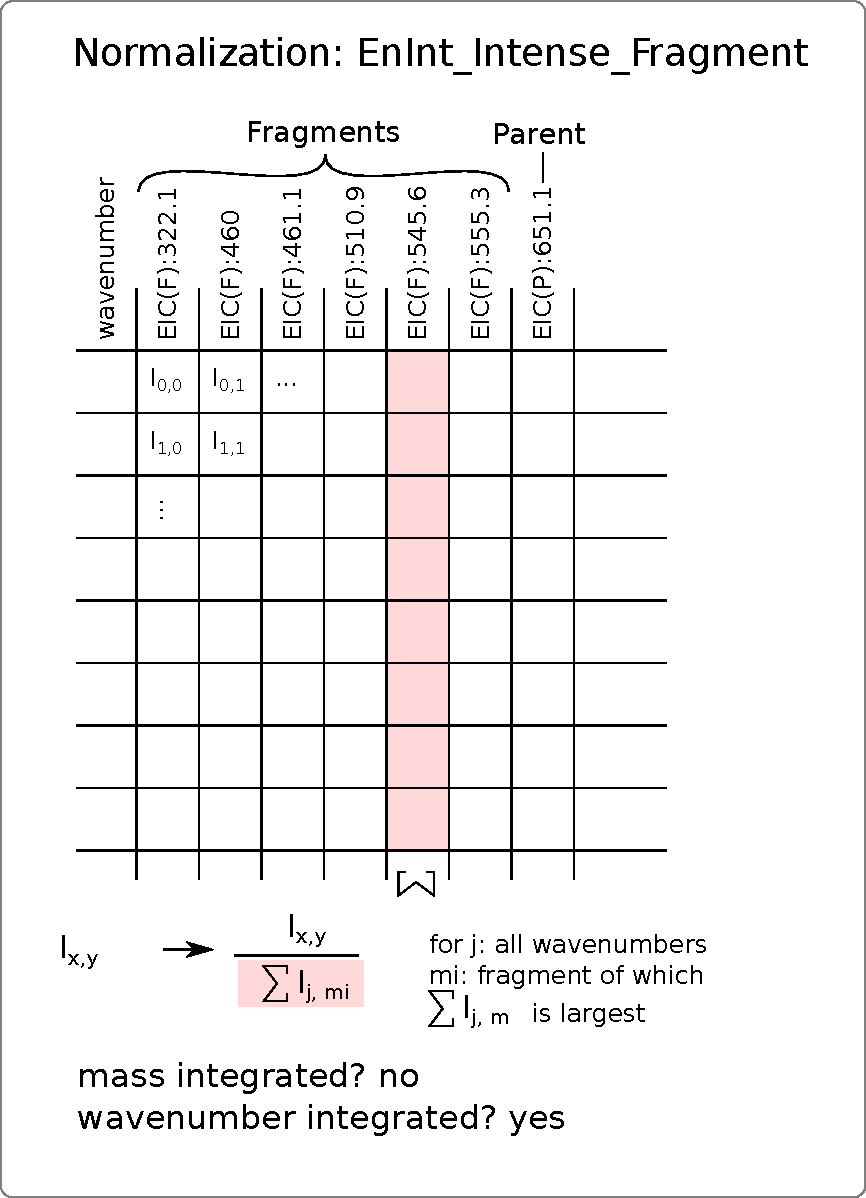
\includegraphics[width=1\linewidth]{../Graphics/Normalization/Normalization_visual_EnInt_Intense_Fragment.pdf}
		\label{fig:MetEnk_sequence_notation}
	\end{subfigure}
	\begin{subfigure}{.25\textwidth}
		\centering
		\includegraphics[width=1\linewidth]{../Graphics/Normalization/Normalization_visual_EnInt_Largest_fragment.pdf}
		\label{fig:MetEnk_sequence_notation}
	\end{subfigure}
\\
	\begin{subfigure}{.25\textwidth}
		\centering
		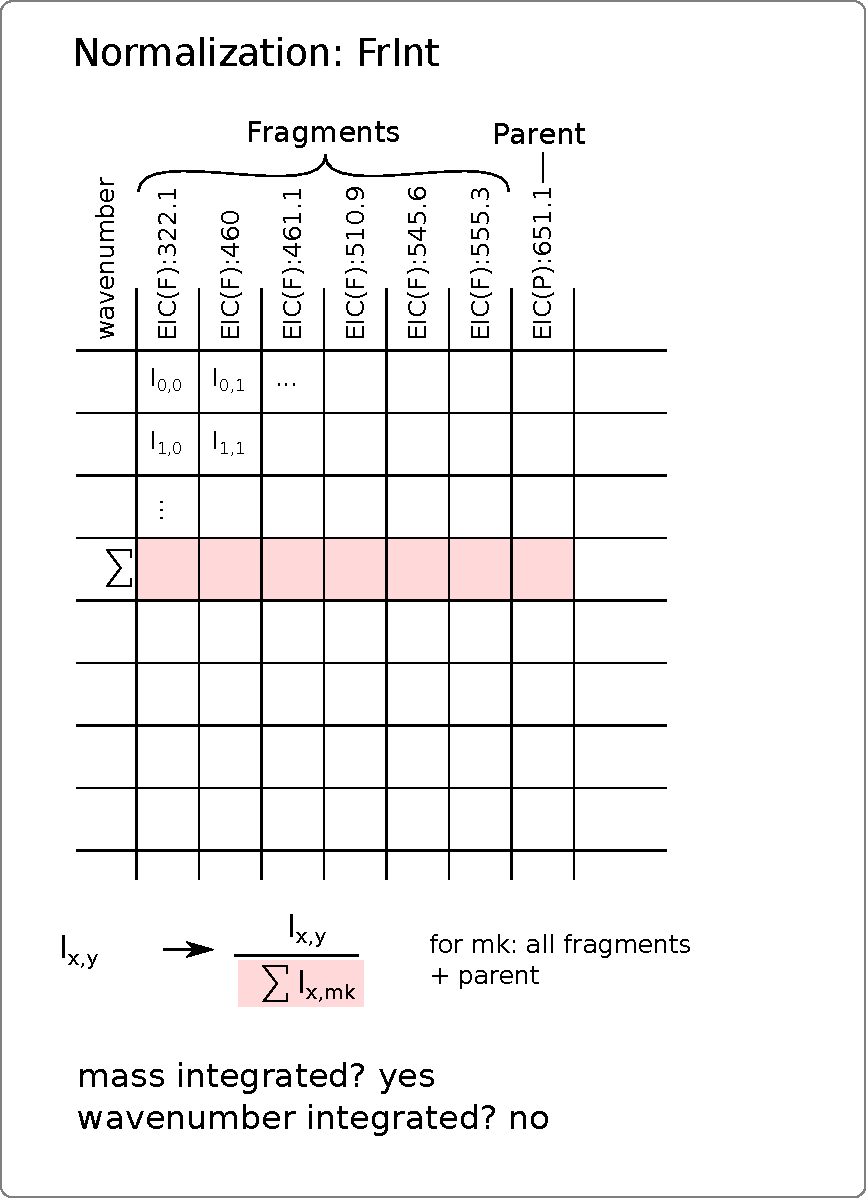
\includegraphics[width=1\linewidth]{../Graphics/Normalization/Normalization_visual_FrInt.pdf}
		\label{fig:MetEnk_sequence_notation}
	\end{subfigure}
	\begin{subfigure}{.25\textwidth}
		\centering
		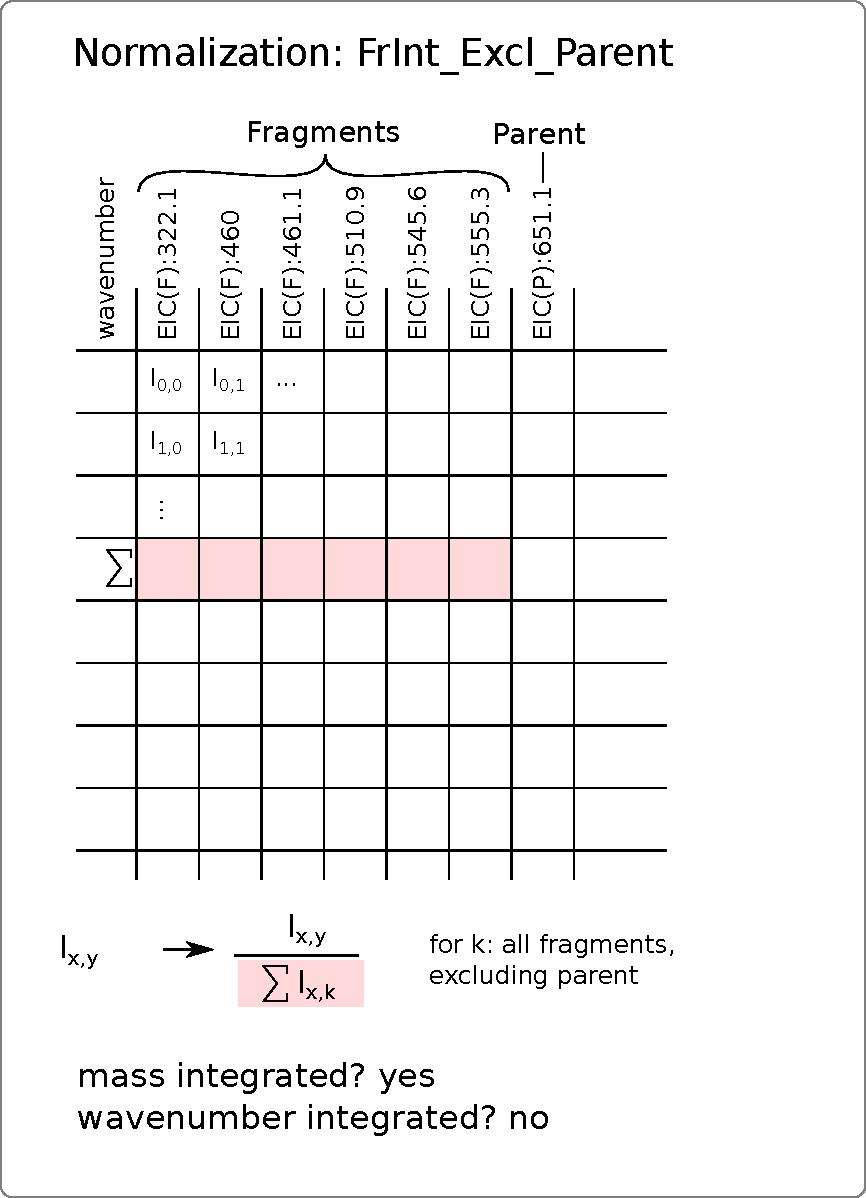
\includegraphics[width=1\linewidth]{../Graphics/Normalization/Normalization_visual_FrInt_Excl_Parent.pdf}
		\label{fig:MetEnk_sequence_notation}
	\end{subfigure}
	\begin{subfigure}{.25\textwidth}
		\centering
		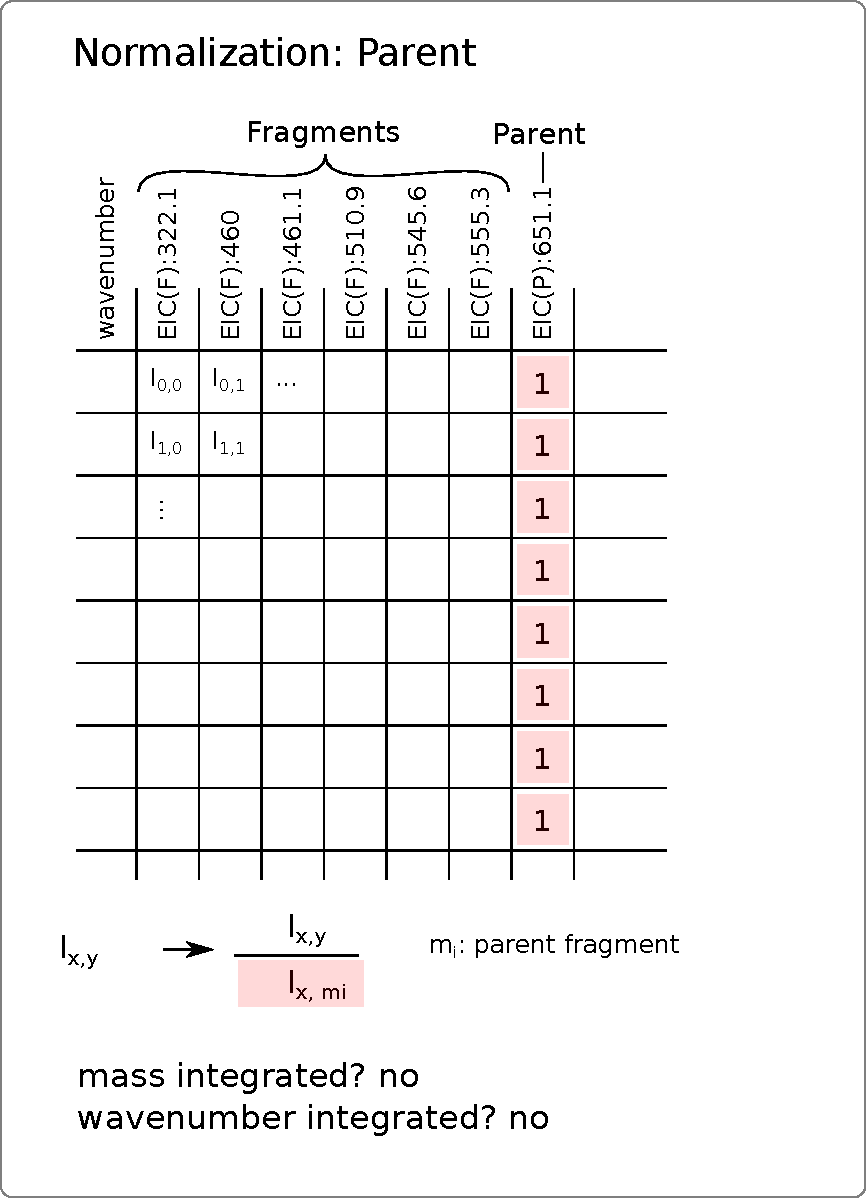
\includegraphics[width=1\linewidth]{../Graphics/Normalization/Normalization_visual_Parent.pdf}
		\label{fig:MetEnk_sequence_notation}
	\end{subfigure}
\\
	\begin{subfigure}{.25\textwidth}
		\centering
		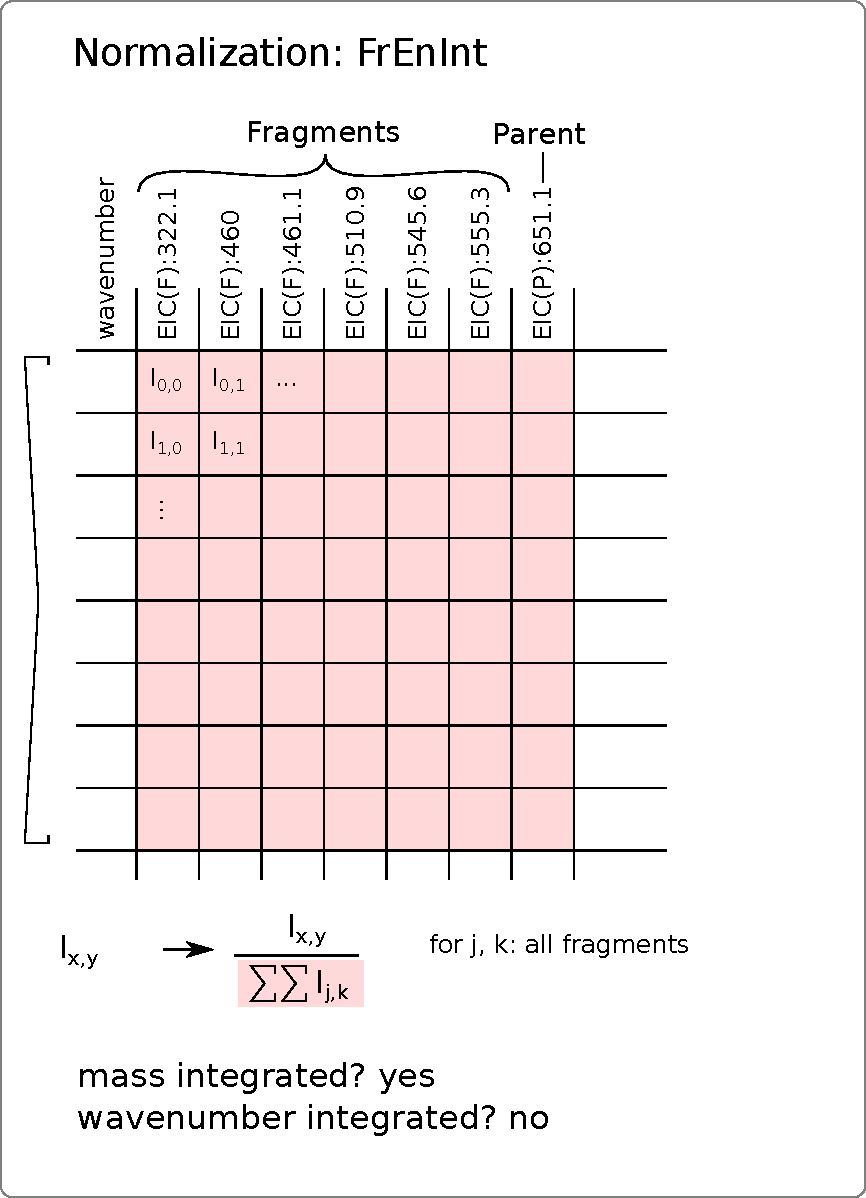
\includegraphics[width=1\linewidth]{../Graphics/Normalization/Normalization_visual_FrEnInt.pdf}
		\label{fig:MetEnk_sequence_notation}
	\end{subfigure}
	\begin{subfigure}{.3\textwidth}
		\centering
		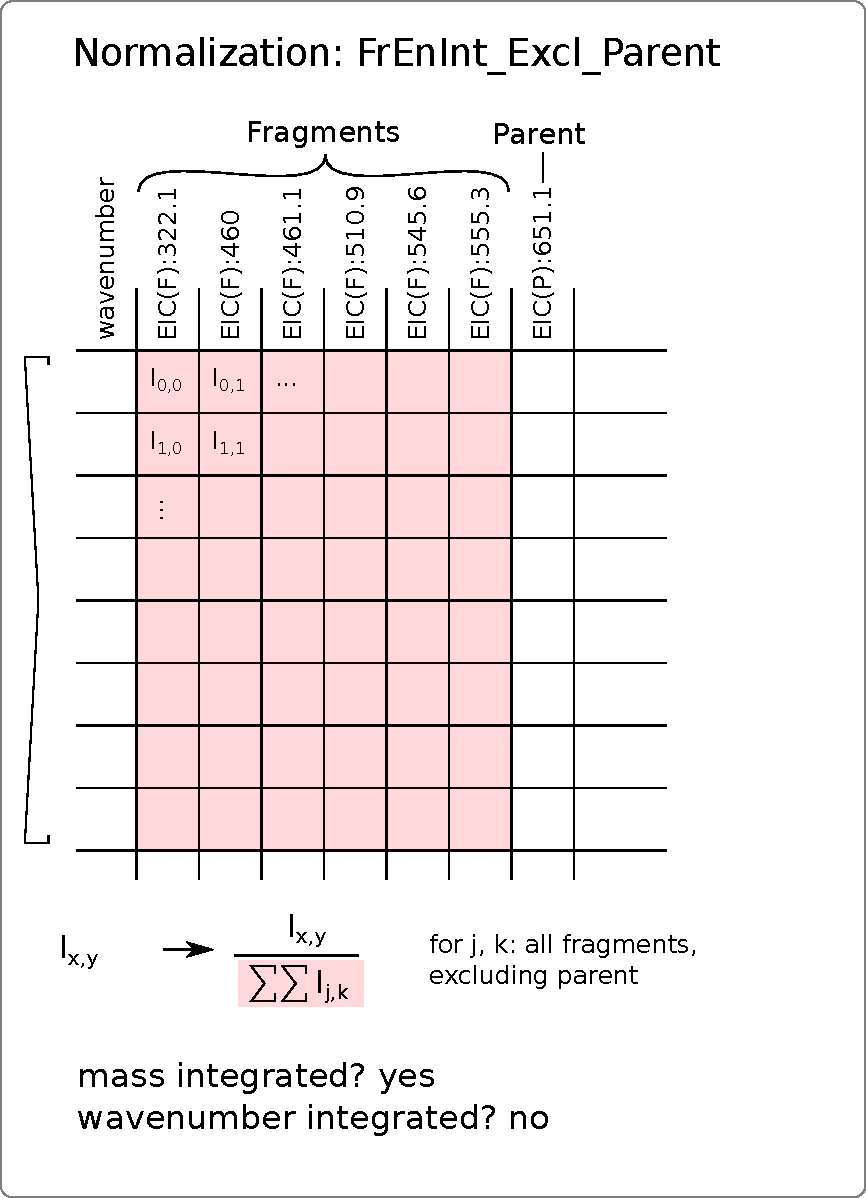
\includegraphics[width=1\linewidth]{../Graphics/Normalization/Normalization_visual_FrEnInt_Excl_Parent.pdf}
		\label{fig:MetEnk_sequence_notation}
	\end{subfigure}
\caption{The Normalization schemes to choose from. 'Fr' is an abbreviation of 'Fragment', 'Int' stands for 'Integrated', 'Wvnr' stands for 'Wavenumber', 'En' stands for (photon) 'Energy' (or wavenumber)}
\end{figure}